\documentclass[12pt]{article}
\usepackage[margin=1in]{geometry}
\usepackage{amsmath,amsfonts,graphicx}
\usepackage{cite}
\usepackage{hyperref}
\usepackage{listings}
\usepackage{color}
\usepackage{times}

\title{ENEL 625 - (Winter 2025) - Estimation Theory \\ Kalman Filtering for Sparse Signals}
\author{Alireza Esmaeili \\ UCID: 30168899 \\ Instructor: Professor Dimitrov \\ \includegraphics[height=12pt]{github-mark.png}~\href{https://github.com/alireza-es/kalman-sparse-filtering}{github.com/alireza-es/kalman-sparse-filtering}}
\date{\today}

\begin{document}

\maketitle

\begin{abstract}
This report investigates the application of Kalman filtering to sparse signal estimation in linear dynamic systems. We explore how incorporating sparsity constraints improves performance over standard Kalman filtering. A simulation study demonstrates the effectiveness of a simple thresholding-based modification.
\end{abstract}

\section{Introduction}
Modern signal processing often involves high-dimensional state estimation, where only a few components are active at any given time. These \textit{sparse signals} appear in applications such as compressed sensing, wireless communications, neuroscience, and target tracking.

The Kalman filter is a powerful algorithm that provides optimal recursive state estimates in linear-Gaussian systems. However, standard Kalman filtering does not explicitly account for sparsity, potentially reducing estimation accuracy when the true state is sparse.

In this project, we investigate the effect of sparsity-aware modifications on Kalman filter performance. Specifically, we integrate a simple thresholding technique within the Kalman filter loop and evaluate its ability to track sparse time-varying signals under noise. The study includes theoretical modeling, Python implementation, and detailed performance analysis.

\section{Problem Description and Formulation}
In this project, we focus on estimating sparse time-varying state vectors in a linear dynamic system using a modified Kalman filter. Sparse signals are defined by the fact that most of their components are zero or negligible, a property common in many real-world applications such as target tracking, neural signal processing, and wireless channel estimation.

The main challenge lies in accurately recovering the underlying sparse signal from a limited number of noisy observations. In our formulation, the state-space model consists of the following linear equations:
\begin{align}
    x_k &= A x_{k-1} + w_k, \\
    y_k &= H x_k + v_k,
\end{align}
where $x_k \in \mathbb{R}^n$ is the hidden sparse state vector at time step $k$, $y_k \in \mathbb{R}^m$ is the measurement vector, $A$ is the state transition matrix, and $H$ is the observation matrix. The process noise $w_k \sim \mathcal{N}(0, Q)$ and measurement noise $v_k \sim \mathcal{N}(0, R)$ are assumed to be zero-mean Gaussian white noise with known covariance matrices.

The estimation objective is to recursively compute an accurate estimate $\hat{x}_k$ of the true sparse state $x_k$ given the sequence of observations $\{y_1, y_2, \dots, y_k\}$.

Standard Kalman filtering assumes Gaussianity and full support of the state vector, leading to dense estimates that are not optimal for sparse systems. We propose a modified approach where a sparsity-enforcing thresholding step is applied after each Kalman update, effectively zeroing out small-magnitude components and improving sparsity consistency.

This formulation allows us to assess how well this modification balances estimation accuracy and sparsity enforcement under various noise and sparsity scenarios.

\section{Mathematical Background}
The Kalman filter is a recursive estimator designed for linear systems with Gaussian noise. It estimates the state of a system by combining prior knowledge (prediction) with new incoming measurements (update).

\subsection{Linear System Model}
We consider the standard discrete-time linear system:
\begin{align}
    x_k &= A x_{k-1} + w_k, \\
    y_k &= H x_k + v_k,
\end{align}
where:
\begin{itemize}
    \item $x_k \in \mathbb{R}^n$ is the state vector at time $k$
    \item $y_k \in \mathbb{R}^m$ is the observation vector
    \item $A$ is the state transition matrix
    \item $H$ is the observation matrix
    \item $w_k \sim \mathcal{N}(0, Q)$ is the process noise
    \item $v_k \sim \mathcal{N}(0, R)$ is the measurement noise
\end{itemize}

\subsection{Kalman Filter Equations}
The Kalman filter operates in two steps:

\textbf{1. Prediction Step:}
\begin{align}
    \hat{x}_{k|k-1} &= A \hat{x}_{k-1|k-1}, \\
    P_{k|k-1} &= A P_{k-1|k-1} A^T + Q
\end{align}

\textbf{2. Update Step:}
\begin{align}
    K_k &= P_{k|k-1} H^T (H P_{k|k-1} H^T + R)^{-1}, \\
    \hat{x}_{k|k} &= \hat{x}_{k|k-1} + K_k (y_k - H \hat{x}_{k|k-1}), \\
    P_{k|k} &= (I - K_k H) P_{k|k-1}
\end{align}

\subsection{Assumptions}
The Kalman filter assumes:
\begin{itemize}
    \item Linear system dynamics
    \item Gaussian white noise for both process and measurements
    \item Known matrices $A$, $H$, $Q$, and $R$
\end{itemize}

Under these assumptions, the Kalman filter is the optimal estimator in the minimum mean squared error (MMSE) sense.

\section{Proposed Method}

To enhance the performance of the Kalman filter for sparse signal estimation, we introduce a sparsity-enforcing mechanism after the standard update step. This modification involves applying a hard-thresholding operation to the state estimate vector, setting small-magnitude elements to zero.

\subsection{Motivation}
In traditional Kalman filtering, all components of the state vector are treated equally. When the true state is sparse, this results in estimates that often include small non-zero entries where the actual value should be zero. By enforcing sparsity explicitly, we aim to reduce estimation noise and improve interpretability.

\subsection{Modified Kalman Filter with Thresholding}
After the standard Kalman update:
\begin{equation}
    \hat{x}_{k|k} = \hat{x}_{k|k-1} + K_k (y_k - H \hat{x}_{k|k-1}),
\end{equation}
we apply a thresholding step:
\begin{equation}
    \hat{x}_{k|k}^{(\text{thresh})}[i] =
    \begin{cases}
    \hat{x}_{k|k}[i], & \text{if } |\hat{x}_{k|k}[i]| \geq \tau \\
    0, & \text{otherwise}
    \end{cases},
\end{equation}
where $\tau$ is a manually selected threshold parameter.

\subsection{Algorithm Summary}
\begin{enumerate}
    \item Initialize $\hat{x}_{0|0}$ and $P_{0|0}$
    \item For each time step $k = 1, ..., T$:
    \begin{itemize}
        \item Predict: $\hat{x}_{k|k-1} = A \hat{x}_{k-1|k-1}$
        \item Predict Covariance: $P_{k|k-1} = A P_{k-1|k-1} A^T + Q$
        \item Compute Kalman gain: $K_k = P_{k|k-1} H^T (H P_{k|k-1} H^T + R)^{-1}$
        \item Update: $\hat{x}_{k|k} = \hat{x}_{k|k-1} + K_k (y_k - H \hat{x}_{k|k-1})$
        \item Threshold: $\hat{x}_{k|k}^{(\text{thresh})} = \text{Threshold}(\hat{x}_{k|k}, \tau)$
        \item Update Covariance: $P_{k|k} = (I - K_k H) P_{k|k-1}$
    \end{itemize}
\end{enumerate}


\section{Simulation Setup}

To evaluate the proposed sparsity-aware Kalman filtering method, we simulate a linear dynamic system with sparse states. A custom Python notebook is used to generate the true sparse state vectors and corresponding noisy observations.

\subsection{Simulation Configuration}
The system consists of:
\begin{itemize}
  \item Time steps: 50
  \item State dimension: 20
  \item Measurement dimension: 10
  \item Sparsity level: 5 non-zero state variables
  \item Transition matrix: Identity matrix ($A = I_n$)
  \item Observation matrix: Gaussian random matrix ($H \in \mathbb{R}^{10 \times 20}$)
  \item Process noise covariance: $Q = 0.01 \cdot I_n$
  \item Observation noise covariance: $R = 0.1 \cdot I_m$
\end{itemize}

\subsection{Sparse Signal Generation}
The non-zero entries in the state vector remain fixed over time and evolve via a random walk process. All other components remain zero. This models a realistic sparse signal, common in applications like compressed sensing, neuroscience, and wireless channel estimation.

\subsection{Python Implementation}
The simulation is implemented in a Jupyter notebook using NumPy for computation and Matplotlib for visualization.

\subsection{Code and Data Access}
The GitHub repository includes:
\begin{itemize}
  \item \textbf{Notebook folder:} \href{https://github.com/alireza-es/kalman-sparse-filtering/tree/main/notebooks}{github.com/alireza-es/kalman-sparse-filtering/notebooks}
  \item \textbf{Data folder:} \href{https://github.com/alireza-es/kalman-sparse-filtering/tree/main/data}{github.com/alireza-es/kalman-sparse-filtering/data}
  \item \textbf{Plots folder:} \href{https://github.com/alireza-es/kalman-sparse-filtering/tree/main/plots}{github.com/alireza-es/kalman-sparse-filtering/plots}
\end{itemize}

These files serve as the foundation for the following Kalman filter-based estimation methods explored in the next sections.

\section{Results and Discussion}

\subsection{True Sparse Signal Visualization}

\begin{figure}[h!]
  \centering
  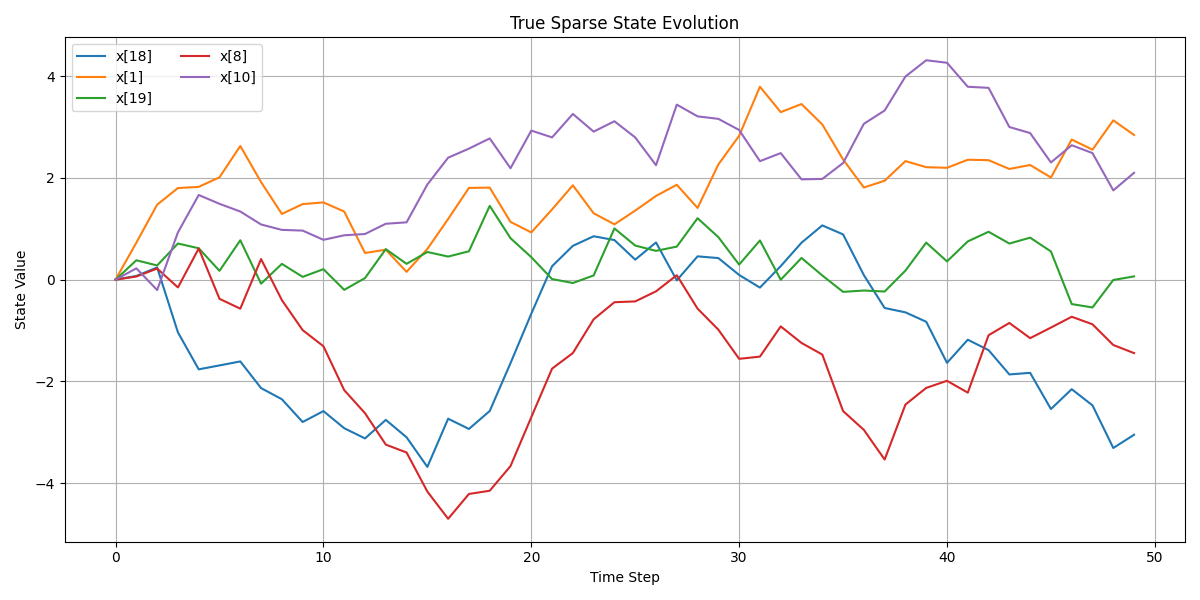
\includegraphics[width=\linewidth]{true_sparse_states.png}
  \caption{True sparse state evolution over 50 time steps. Only the active state components are shown.}
  \label{fig:sparse-true}
\end{figure}

\subsection{Standard Kalman Filter Performance}
Figure~\ref{fig:kf-standard} shows the comparison between the estimated states and the true sparse states for the active components. Dashed lines represent the true state values, while solid lines show the values estimated by the Kalman filter.

\begin{figure}[h!]
  \centering
  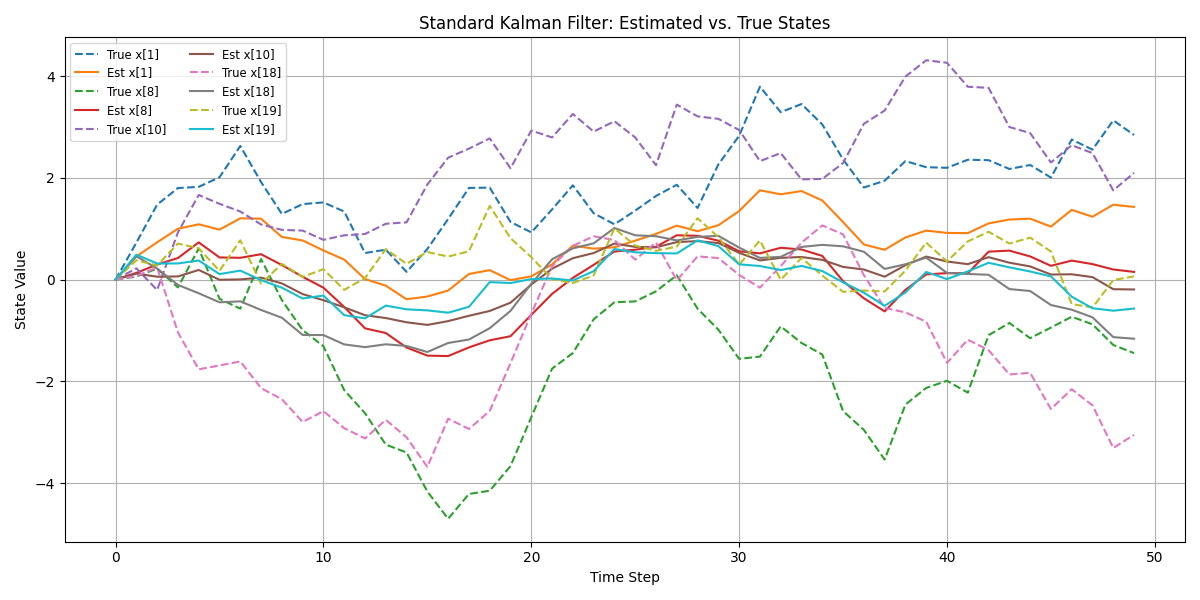
\includegraphics[width=\linewidth]{kf_est_vs_true.png}
  \caption{Standard Kalman Filter: Estimated vs. True sparse states. Dashed lines indicate true state components; solid lines are the Kalman filter estimates.}
  \label{fig:kf-standard}
\end{figure}

As seen in the plot, the Kalman filter can roughly follow the trajectory of active components but suffers from the following issues:

\begin{itemize}
  \item Small estimation errors, particularly in dynamic transitions
  \item Non-zero estimations for components that should remain zero (lack of enforced sparsity)
  \item Smoothing effect that reduces the sharpness of transitions
\end{itemize}

While effective in tracking general trends, the standard Kalman filter introduces noise in zero-expected components, indicating the need for a sparsity-enforcing mechanism to suppress irrelevant fluctuations.

\section{Conclusion}

% To be written at the end of analysis.

\begin{thebibliography}{1}
\bibitem{vaswani2008}
N. Vaswani, ``Kalman filtered compressed sensing,'' in 	extit{Proc. ICIP}, 2008.

\bibitem{carmi2010}
A. Carmi, P. Gurfil, and D. Kanevsky, ``Methods for sparse signal recovery using Kalman filtering,'' 	extit{IEEE Transactions on Signal Processing}, vol. 58, no. 4, pp. 2405--2409, Apr. 2010.
\end{thebibliography}

\end{document}
